\section{Motivation}\label{sec:background}

\aditya{updated the leadin to be less generic. ptal}
 OS policies' decisions are often driven by approximate information, such as values estimated from offline profiling, predictions from learned models, or heuristics tuned for a particular workload or machine regime. These signals can guide good decisions when deployment-time conditions resemble the setting for which the policy was designed. But when workloads, inputs, or hardware conditions shift, the same signals may no longer aling with what the policy actually needs to optimize. The upshot is that (a) performance may regress, and (b) the regression is often hard to attribute to any particular decision logic or design assumption.

We make this concrete through two representative examples. The first, CBMM, shows how a policy built around offline benefit estimates can become misaligned with current execution behavior. The second, FLUX, shows the analogous issue for learned policies, where the model may continue to produce outputs even when its inputs no longer match the regime in which it was trained. We then broaden the discussion to show that this is not limited to these two systems, but appears across several OS subsystems. The goal of this section is to isolate the common structure behind these examples and motivate the need for a more systematic approach.

\iffalse 
\aditya{this lead in needs to be completely rewrittent to be technically sound and it needs citations. it is also broken and does not tie the intro to what follows.}
Conventionally, OS policies have relied on broad, fairly stable assumptions: that workloads exhibit similar locality patterns, that hardware behavior can be summarized by a small set of predictable trends, and that performance tradeoffs profiled once will remain valid across deployments. \eric{citations? examples?}
% While this single policy was still not optimal, it was optimal to use it for general-purpose applications \ds{why?}.
While such one-size-fits-all policies were rarely optimal for every application, they were a reasonable compromise for general-purpose systems, where broad applicability and robustness mattered more than per-workload optimality. \eric{does it make sense to call out the emphasis on tail latency here? Or is that a distraction?}
However, recent trends suggest that these assumptions break down more often in modern environments, where applications have diverse requirements, and both workloads and hardware evolve rapidly over time. \eric{citations needed}
\fi


\subsection{Brittle Assumptions in Modern OS Policies}

In this section, we provide two examples to demonstrate how policies designed under certain assumptions can fail when those assumptions break at deployment time. These examples motivate the need for a common framework for monitoring such assumptions at run-time and responding when they break. We will revisit these examples in \Cref{sec:case-studies} to show how guardrails can be used to address these challenges in practice.

\begin{figure}[t]
    \centering
    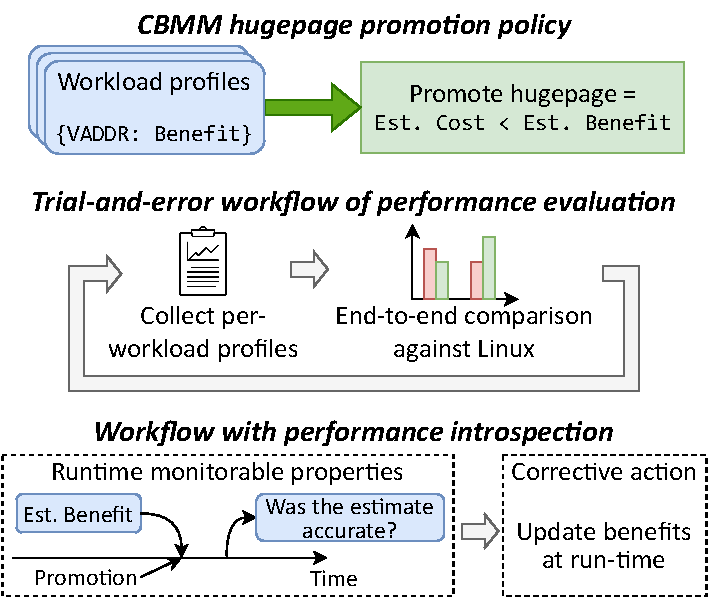
\includegraphics[width=0.9\columnwidth]{figures/Examples/CBMM-example.pdf}
    \caption{Challenges with offline evaluation for CBMM and a workflow based on run-time performance introspection.}
    \label{fig:cbmm-example}
\end{figure}


\paragraph{Hugepage Promotion in CBMM.}
Consider a hugepage-promotion policy based on Cost-Benefit Memory Management (CBMM)~\cite{cbmm-atc22}. Hugepages can reduce TLB pressure and improve address-translation performance, but promoting them also incurs nontrivial allocation and compaction costs. CBMM uses the observation that Linux promotes hugepages too aggressively, and instead, only promotes a hugepage when its estimated benefit exceeds its estimated cost. In particular, the policy uses offline profiling to estimate how much benefit a given page region is likely to obtain from promotion, and combines that estimate with run-time cost signals to decide whether promotion is worthwhile.

\aditya{do we have any empirical results to back this up? we seem to refer to it later} The challenge is that the estimated benefit is only as good as the assumptions underlying the offline profile. As memory access patterns shift or as interference from co-located processes changes the memory fragmentation, the page regions that, according to the profile, would benefit most from hugepage promotion may no longer be the right ones to promote. Thus, the policy may end up operating on stale assumptions and make worse decisions.

Today, detecting such regressions requires extensive end-to-end comparisons between CBMM and baselines across multiple workloads. Even then, poor performance only shows that the policy regressed, but it does not immediately explain why or how to improve it.
This example illustrates the need for three capabilities. First, the system must be able to monitor {\em a run-time signal} that reveals when the profiled benefit estimates are no longer trustworthy. Second, it must be able to associate such a failure with {\em an appropriate response}, such as updating the benefit estimates online or falling back to a more conservative promotion policy. Finally, it must provide a way to relate such a local intervention to the higher-level objective the operator actually cares about, such as producing good promotion decisions. 

\begin{figure}
    \centering
    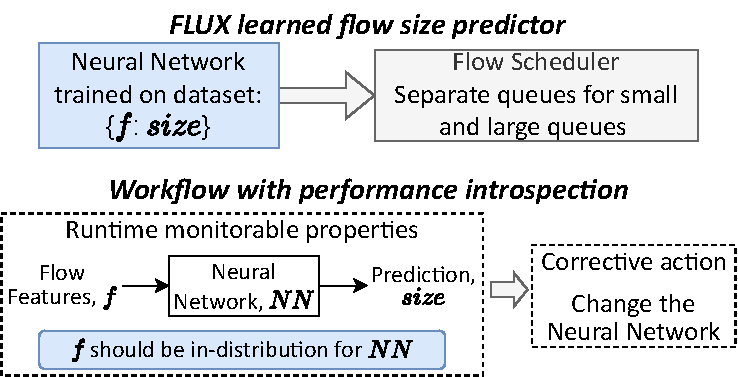
\includegraphics[width=0.9\columnwidth]{figures/Examples/FLUX-example.pdf}
    \caption{Challenges with policies using learned models and a workflow based on performance introspection.}
    \label{fig:flux-example}
\end{figure}

\paragraph{Learned Flow Scheduling using FLUX.}
As a second example, consider FLUX~\cite{flux-nsdi19} (\Cref{fig:flux-example}), a learned flow scheduler that predicts the size of each new flow and uses that prediction for scheduling. Such predictions can be highly useful because short flows are often latency-sensitive, and scheduling them aggressively can substantially improve completion times. But the quality of this decision depends directly on the quality of the prediction model. In particular, FLUX assumes that the features seen at deployment time resemble those on which the model was trained.

\aditya{do we have any empirical results to back this up?}
This assumption can easily fail in practice. The distribution of features may shift as the mix of applications changes, as deployment conditions differ from the training environment, or as the model encounters flows from workloads that were underrepresented in the original training data. In these cases, the predictor may continue to produce outputs for every flow, but those outputs may no longer be reliable enough to support good scheduling decisions. The scheduler quietly continues to operate while making increasingly poor decisions.

This example highlights a complementary challenge. For learned policies, the relevant run-time signal may concern not only the quality of the eventual decisions, but also whether the model is being applied within the regime for which it was trained. The system must therefore support checks over model inputs or outputs, corrective actions such as switching predictors or reverting to a default scheduler, and a way to connect these local responses to the scheduler's higher-level performance objective.


\subsection{A Pervasive Problem}
These issues arise throughout the OS. For example, consider the Linux kernel page cache policy: {\tt cache_ext}~\cite{cache-ext-sosp25} demonstrates that the best-performing eviction heuristic changes for different workloads: while LFU results in the best throughput for YCSB traces, the study reports that for Twitter traces, LFU is seldom the optimal, and the best performing heuristic can vary between S3-FIFO~\cite{s3fifo-sigcomm}, MGLRU, and LHD.
Thus, choosing the eviction policy based on the performance of just one workload may result in sub-optimal performance on other workloads.

As another example, consider the problem of dispatching I/O requests to SSD devices.
LinnOS~\cite{linnos-osdi20} proposes a learning-based model to predict the I/O latencies, reporting high accuracy and low inference overhead on the devices and traces it studied.
However, it was later reported~\cite{heimdall-eurosys25} that the performance of the LinnOS model degraded to only 67\% accuracy on faster devices. %\aditya{drop the rest of this sentence. this seems like a dig at the linnos authors. do we want to say this?} that were, notably, released around the same time frame as the devices studied by LinnOS.
Thus, even sophisticated policy can be tightly coupled to particular hardware characteristics that evolve over time, and change from vendor to vendor.

% \ds{Add the argument that this guardrail-style of policy development has been applied previously, but in an ad-hoc manner -- we provide a framework to do it in a principled way.}
% \eric{i think this can go in the related work section.}

% \sujay{We could add some examples motivating need for perf introspection. Why is it more important today than before? I can think of 2 reasons: 1) learned policies, understanding the behavior of which is more difficult, and 2) instance-optimal heuristics which may work well for one workload but perform poorly for another. We could add examples or some data for this.}


\subsection{The Power of Performance Introspection}

\aditya{simplified this lead out}

The examples above point to a common need: many OS policies rely on proxies such as profiles, predictions, or heuristics, and those proxies can become unreliable at deployment time. We need a way to identify, during execution, when that happens and how the system should respond.

In particular, a reusable, common framework is called for because otherwise each policy must implement its own monitoring and repair logic in an ad hoc way. Such bespoke mechanisms are difficult to implement, compare, and connect to a clear performance objective.


Performance introspection addresses this gap by making these elements explicit within a single OS-level abstraction. The challenge is that a general OS framework must accommodate diverse policies, kernel-visible signals, low-overhead monitoring/enforcement, and explicit links between local checks and higher-level performance goals to ensure trustworthiness. In this sense, our proposed framework is close in spirit to monitor-oriented programming~\cite{oopsla07} and aspect-oriented programming~\cite{kiczales1997aspect}, but is specialized to OS-specific performance conditions, online corrective actions, and their connection to higher-level performance objectives. Many prior OS policy designs already contain fragments of this pattern in policy-specific form~\cite{}, \aditya{needs citations; perhaps add darwin, percs} with bespoke checks and repairs embedded directly into the mechanism. We elevate that recurring pattern into a principled framework.

\eric{How do we point to the cool fact that we have a general framework in the OS, despite the fact that its hard?}

\ds{Perhaps here we can add that other OS policy papers also tend to use guardrails as checks, but it is ad-hoc. @Sujay: pls help.} \aditya{added a placeholder sentence but that needs refinement}


\iffalse 
\aditya{i don't buy this networking analogy at all. those are control systems - and all control systems have an observer and control logic. guardrails are not a control system, but they augment a control system. the current lead in can therefore confuse a reviewer. do we have a different example?} In the networking domain, research on closed-loop control has shown the value of linking poor performance observations to restorative actions. For example, CONGA~\cite{alizadeh2014conga} and HULA~\cite{katta2016hula} redirect traffic using fast data-plane congestion signals, while HPCC~\cite{li2019hpcc} uses in-band network telemetry to adjust sender rates from precise online feedback. These systems show that live measurements can drive effective performance protection, not just post hoc diagnosis. Unfortunately, each of these systems is a problems specific engineering loop whose signals, actions, and rationale are deeply tied to specific deployments. To make matters worse, this pattern of monitoring and intervention in networking was only enabled by specific hardware support for in-network telemetry and fast data-plane actions, which are not yet widely available in in the OS. 

\eric{How do we point to the cool fact that we have a general framework in the OS, despite the fact that its hard?}

\ds{Perhaps here we can add that other OS policy papers also tend to use guardrails as checks, but it is ad-hoc. @Sujay: pls help.}

Guardrails generalize this pattern: taking inspiration from programming patterns like monitor-oriented programming~\cite{oopsla07} and aspect-oriented programming~\cite{kiczales1997aspect}, Guardrails provide a domain-specific abstraction for pairing performance checks with corrective actions that ensure performance safety. By making the condition, response, and resulting guarantees explicit, Guardrails enable developers to design better and more responsive systems.
\eric{We need something better to conclude}

\fi
